\section{Measurement Infrastructure}
\label{datasets}
These included which vantage points within a country to use, which servers to use as relays, and which method to use for geolocating IP addresses.  We also introduce our measurement methods for measuring where current Internet traffic is traveling to, how well open DNS resolvers help clients avoid specific countries, and how well relays help clients avoid specific countries.

\begin{figure*}
\centering
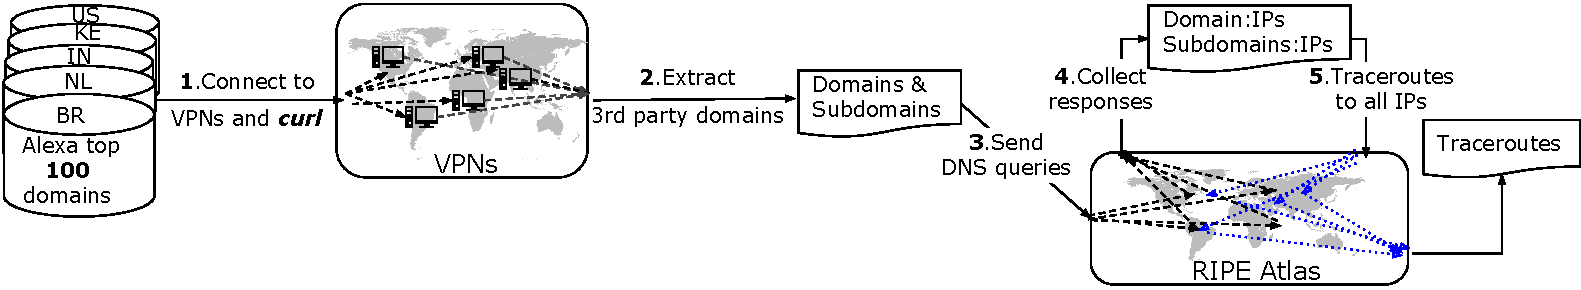
\includegraphics[width=.9\textwidth]{Current-Traffic_fig}
\caption{The measurement pipeline to study current traffic routes.}
\label{fig:pipeline1}
\end{figure*}

\begin{figure}
\centering
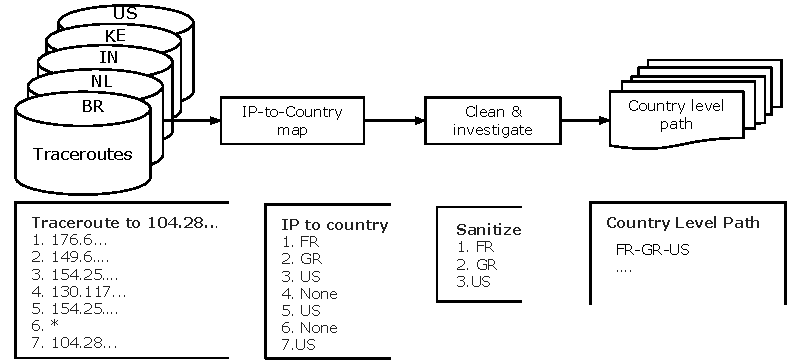
\includegraphics[width=.5\textwidth]{Analysis-Pipeline_fig}
\caption{The measurement pipeline to analyze traceroutes.}
\label{fig:analysis_pipeline}
\end{figure}

\subsection{Measurement Pipelines}
\label{pipeline}
{\bf Current Traffic.} Our methods for measuring where traffic paths go use the data-plane; we analyze the reported hops of traceroute measurements to find which countries are on the path from a client in Country X to a popular domain.  For this study, we used RIPE Atlas probes in Country X, specifically the set of probes that had unique ASes in the country.  The destinations for traceroutes are the Country X Alexa Top 100 domains, as well as the third party domains within the response bodies of the 100 domains.  There are three main steps to our measurement procedure: traceroute generation and collection, transformation of traceroutes to country-level paths, and path analysis.

{\bf Country Avoidance with Open Resolvers.} If content is replicated in different parts of the world, open DNS resolvers located around the globe can potentially help clients circumvent surveillance states.  To measure this, we first pick a set of open resolvers to query, then query with Country X's Alexa Top 100 domains, and traceroute from a client in Country X to the DNS responses given by the open resolvers.  These three steps are explained in more detail below.

{\bf Country Avoidance with Relays.} Using an overlay network may help clients route around unfavorable countries or access content that is hosted in a more favorable country.  First, we select relays that are geographically diverse, run traceroute measurements from Country X to each relay and from each relay to the Country X Alexa Top 100 domains.  Based on these two sets of traceroutes, we can run analyses to determine if they improve country avoidability. 

\subsection{Limitations}
The measurement methods described in Section~\ref{datasets} are not without limitations.  First, our study is solely based on IPv4 routes, which likely differ from IPv6 routes.  Here we also discuss limitations with geolocation accuracy, path asymmetry, and traceroute completeness.

\subsubsection{IPv4}
The measurements we conducted only collect and analyze IPv4 paths, and therefore all IPv6 paths are left out of our study.  IPv6 paths likely differ from IPv4 paths as not all routers that support IPv4 also support IPv6.  Future work includes studying IPv6 paths and which countries they transit, as well as a comparison of country avoidability between IPv4 and IPv6 paths. 

\subsubsection{Country Mapping}
Previous work has shown that there are fundamental challenges in deducing a geographic location from an IP address, despite using different methods such as DNS names of the target, network delay measurements, and host-to-location mapping in conjunction with BGP prefix information~\cite{padmanabhan2001investigation}.  Because the focus of this work is on measuring and avoiding surveillance, and not on geolocation algorithms, we used a pre-existing geolocation service: MaxMind~\cite{maxmind}.

Geolocation services and tools have been studied and proposed, and continue to be a growing research area.  We use MaxMind's geolocation service to map IP addresses to their respective countries.  While it has been shown that there are inaccuracies and incompleteness in MaxMind's data, research has also shown that other geolocation tools have similar or worse inaccuracy rates~\cite{huffaker2011geocompare}.  To address the incompleteness of the data, we cleaned up our IP to country mapping by removing all IP addresses that resulted in a `None' response when querying MaxMind.  This method provides a lowerbound on the number of countries that are included on the path, and therefore a lowerbound on the countries that can conduct surveillance.  

\subsubsection{Path Asymmetry}
Previous work has shown that paths are not symmetric most of the time -- the forward path from point A to point B does not match the reverse path from point B to point A~\cite{he2005routing}.  Most work on path asymmetry has been done at the AS level, but not at the country level.  Our measurement methods only take the forward path (from client to domain or relay) into account, and not the path from the domain or relay to the client.  

We conducted a study to measure path asymmetry at the country granularity; if country-level paths are symmetric, then the results of our measurements would be representative of the forward {\it and} reverse paths, but if the country-level paths are asymmetric, then our measurement results only provide a lowerbound on the number of countries that could potentially conduct surveillance.  Using 100 RIPE Atlas probes located around the world, and 8 Amazon EC2 instances, we ran traceroute measurements from every probe to every EC2 instance and from every EC2 instance to every probe.  After geolocating the IPs to countries, we analyzed the paths for symmetry.  First, we compared the set of countries on the forward path to the set of countries on the reverse path; this yielded about 30\% symmetry.  What we wanted to know is whether or not the reverse path has more countries on it than the forward path.  We measured how many reverse paths were a subset of the respective forward path; this was the case for 55\% of the paths.  

The results of this measurement are not convincing enough to state that country-level paths are symmetric, and therefore our measurements and results represent a lowerbound on the number of countries that transit traffic; our results are a lowerbound on how many unfavorable countries transit a client's traffic.

\subsubsection{Traceroute Accuracy and Completeness}
Our study is limited by the accuracy and completeness of traceroute.  Research has shown that there are a number of anomalies that can occur in traceroute-based measurements~\cite{augustin2006avoiding}, but most traceroute anomalies do not cause an overestimation in surveillance states.  The incompleteness of traceroutes, where a router does not respond, causes our results to be an underestimation of the number of surveillance states, and therefore also provides a lowerbound on surveillance.
